\subsection{Brief overview of the {\it NIKA} camera during the campaign of November 2012}
\label{sec:run_overview}
\begin{table*}
	\begin{center}
	\begin{tabular}{cccc}
	 \hline
         \hline
	& Nov. 21$^{\mathrm{st}}$ & Nov. 22$^{\mathrm{nd}}$ & Nov. 23$^{\mathrm{rd}}$\\
	\hline
	$\tau_{140 \ \mathrm{GHz}}$ & 0.14 & 0.18 & 0.053 \\
	$\tau_{240 \ \mathrm{GHz}}$ & 0.17 & 0.22 & 0.046 \\
	Time range & 8:27 am to 11:43 am & 8:16 am to 12:01 pm & 8:11 am to 10:59 am \\
	Integration time & 2 hrs 29 min & 3 hrs 00 min & 2 hrs 29 min \\
	Unflagged integration time & 50 min & 2 hrs 35 min & 2 hrs 23 min \\
	\hline
	\end{tabular}
	\end{center}
	\caption{Mean zenith opacity, on-source integration time, and period of the day for the three days of the campaign of November 2012. The total integration time is 5 hrs 47 min. The mean opacity ratio is $\tau_{240~\mathrm{GHz}}~/~\tau_{140~\mathrm{GHz}}~\simeq~1.2$}
	\label{tab:table_obs}
	\end{table*}

The {\it NIKA} camera consists of two arrays of Kinetic Inductance Detectors (KIDs) with maximum transmissions at $140$ and $240$~GHz. Ninety percent of the total transmission of the {\it NIKA} bandpasses (see Fig.~\ref{fig:bandpass}) is in the range 127--171~GHz for 140~GHz and 196--273~GHz for 240 GHz bands. The respective angular resolutions (FWHM) are $18.5$ and $12.5$~arcsec with effective fields of view of $1.8 \times 1.8$ and $1.0 \times 1.0$~arcmin. The pitch between pixels is 2.3~mm at 140~GHz and 1.6~mm at 240~GHz. This corresponds to an effective focal plane sampling of 0.77~F$\lambda$ and 0.8~F$\lambda$ at 140 and 240~GHz, respectively. In this particular campaign, the first band ($140$~GHz) was used with $127$ detectors having a mean effective sensitivity of $29$ mJy s$^{1/2}$ per beam ($19$ mJy s$^{1/2}$ per beam for the best $20$\% of all pixels), and the second band ($240$~GHz) had $91$ detectors with a mean effective sensitivity of $55$ mJy s$^{1/2}$ per beam ($37$ mJy s$^{1/2}$ per beam for the best $20$\% of all pixels). This unexpected poor sensitivity and the small number of available detectors for the 240~GHz band is due to the dysfunction of a cold amplifier during this observation campaign. Using only eight detectors of the 240~GHz array, we obtain the expected mean effective sensitivity measured to be $22$ mJy s$^{1/2}$ per beam. Despite the constant improvement in sensitivity over the the last campaigns~\citep{NIKA_2010,NIKA_2011,RFdIdQ}, the sensitivity of the instrument was limited by detector correlated noise coming from electronic and sky noise residuals. For the averaged background during observations, the expected photon noise is 5 mJy s$^{1/2}$ at 140~GHz and 7 mJy s$^{1/2}$ at 240~GHz.

Unlike traditional bolometric instruments, {\it NIKA} uses KIDs. The KIDs are superconducting resonators whose resonance frequency ($\sim$ 1--2.5~GHz) changes linearly with the absorbed optical power \citep[see for example][]{swenson_2010}. Each resonator can be modeled by a complex transfer function in frequency with a real part $I$ (in-phase) and imaginary part $Q$ (quadrature) \citep{grabovskij_2008}. By measuring $I$ and $Q$ at a constant frequency (defined for each detector by the electronics) as a function of time, we can reconstruct the shift of the resonance frequency, as described in \citet{RFdIdQ}. This method allows us to obtain accurate photometry to be better than 10\%.

The KIDs used here are Hilbert dual-polarization designed LEKID pixels \citep[Lumped Element KID;][]{doyle_2008, roesch_2012}, which are realized on 180 $\mu$m and 275 $\mu$m thickness silicon substrate at 240 and 140 GHz, respectively. The detector resistivity is larger than 5000 $\Omega$ cm for both wavelengths. The detectors are cooled down to about 100~mK with a $^4\mathrm{He}$ -- $^3\mathrm{He}$ dilution cryostat. 

More details on the {\it NIKA} prototype setup can be found in~\cite{main_run5}.

\subsection{Observing strategy of the targeted galaxy clusters}
\label{sec:obs_condition}
Galaxy clusters are weak extended sources when seen through the tSZ effect, making their observations challenging.
For this study, we have selected \mbox{RX~J1347.5-1145}, which is an intermediate redshift cluster at $z = 0.4516$.
 The object \mbox{RX~J1347.5-1145} is among the most luminous tSZ sources in the sky, and
 it is also compact enough to have an angular size comparable to the field of view of the NIKA camera. 

As shown in Fig.~\ref{fig:scans}, the cluster signal is scan-modulated but there is no wobbling involved. Raster scans are made of constant elevation subscans or constant azimuth subscans. For the latter, only the low azimuth part of the field was covered due to an error in the control software. Both of them are $6$ min $20$s scans that are made of $19$ subscans separated by $10$~arcsec steps. Scans along the azimuth direction are centered at (R.A.,~Dec)~=~(13h~47m~32s,~-11$^{\mathrm{o}}$~45'~42"), which sample a rectangular region of $360 \times 180$~arcsec (azimuth $\times$ elevation), while scans along the elevation sample a region of $180 \times 180$~arcsec and are centered on a point $90$~arcsec away from (13h~47m~32s,~-11$^{\mathrm{o}}$~45'~42"), which rotates with the parallactic angle. The scan velocity is about 15~arcsec s$^{-1}$. The detailed integration times are given in Table~\ref{tab:table_obs} with the corresponding atmospheric opacities.
	\begin{figure}
	\centering
	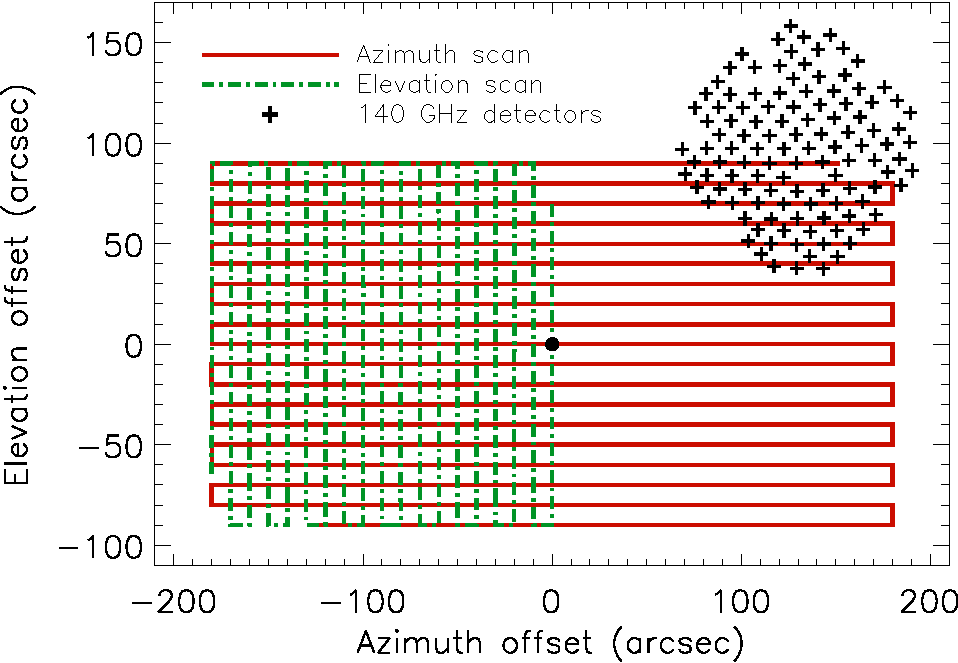
\includegraphics[width=\columnwidth]{Figure/scan}
	\caption{Elevation (dashed green) and azimuth (solid red) offset scans. The center is represented by a black dot and has coordinates (R.A.,~Dec)~=~(13h~47m~32s,~-11$^{\mathrm{o}}$~45'~42"). The 140~GHz array is also represented by black crosses, which correspond to the position of each KID in the focal plane (gaps in the array correspond to invalid detectors).}
        \label{fig:scans}
	\end{figure}
	
\subsection{Pointing, calibration, bandpasses, and beam}
\label{sec:calib_pointing}
Uranus observations were used to reconstruct beam maps (projection of the array on the sky and measure of individual detector beams) for both wavelenghts. Nearby quasars were used for determining pointing corrections. The pointing root mean square error is estimated to be $\sim$3~arcsec \citep{main_run5}. This is small compared to the beam and has a negligible impact in the case of extended sources such as \mbox{RX~J1347.5-1145}.

We also used Uranus for absolute point source flux calibration. The flux of the planet was inferred from a frequency dependent model of the planet brightness temperature taken from \cite{moreno2010}. The Uranus brightness temperatures are typically 113~K at 140~GHz and 94~K at 240~GHz. This model is integrated over the {\it NIKA} bandpasses for each channel, and it is assumed to be accurate at the 5\% level. The final absolute calibration factor is obtained by fitting the amplitude of a Gaussian function of fixed angular size on the reconstructed maps of Uranus (representing the main beam). We neglect the angular diameter of Uranus, 3.54~arcsec at the time of the observations, when it is compared to the size of the main beam, since the convolution of the corresponding disk with a Gaussian of 12.5 and 18.5~arcsec full width at half maximum (FWHM) broadens our beam by only 0.17~arcsec at 240~GHz and 0.12~arcsec at 140~GHz.

Scales larger than 180~arcsec, which correspond to the scan size, were not measured with {\it NIKA}. By integrating the Uranus flux up to 100~arcsec, we observe that the total solid angle covered by the beam, which includes the power in the side lobes, is larger than the Gaussian best-fit of the main beam by a factor of 1.32. Scales larger than 100~arcsec are noise dominated on the Uranus map. Thus, using recent measurements of the IRAM 30-meter beam pattern with EMIR \citep{K13}, we extrapolate the angular profile of the beam from 100~arcsec to 180~arcsec, and find an overall factor equal to 1.45 \citep[see][for a more detailed description]{main_run5}. From the dispersion over different observations of Uranus, we estimate the uncertainties on the solid angle of the main beam to be about 4 \%.  We obtain 10 \% uncertainties for the full beam by also considering uncertainties on the side lobes. 

The sky maps (also for Uranus maps prior to calibration) are corrected for atmospheric absorption using elevation scans, or skydips \citep[see][for further details]{main_run5}. In our case, the resonance frequencies of the detectors are measured versus the optical load, which depends on the zenith opacity and the elevation. This gives the zenith opacity as a function of the resonance frequency of the detectors, which is measured for each scan. The opacity can then be corrected to good accuracy by accounting for the air mass at the elevation of the source. Furthermore, different atmospheric conditions lead to changes in the beam pattern of the instrument that also affect the absolute calibration accuracy \citep{main_run5}. From the dispersion of the recovered flux of Uranus, which was observed several times with different opacities during the campaign, we estimate an overall accuracy of 15\% \citep{main_run5} for the calibration procedure.

To summarize, the list of the main systematic uncertainties in the 140~GHz band are listed in Table~\ref{tab:table_err}. The total calibration uncertainty on the final data at the map level is estimated to be 16\%.
\begin{table}
\begin{center}
\begin{tabular}{cc}
\hline
\hline
Systematic uncertainty & Error percentage \\
\hline
Brightness temperature model & 5\% \\
Point source calibration & 15\% \\
Secondary beams fraction & 45\% $\pm$ 10 \% \\
Bandpasses & 2\% \\
\hline
\end{tabular}
\end{center}
\caption{Main contributions to the absolute error of the {\it NIKA} data for the 140 GHz band.}
\label{tab:table_err}
\end{table}
